% Copyright (c) 2020 Carl Martin Ludvig Sinander.

% This program is free software: you can redistribute it and/or modify
% it under the terms of the GNU General Public License as published by
% the Free Software Foundation, either version 3 of the License, or
% (at your option) any later version.

% This program is distributed in the hope that it will be useful,
% but WITHOUT ANY WARRANTY; without even the implied warranty of
% MERCHANTABILITY or FITNESS FOR A PARTICULAR PURPOSE. See the
% GNU General Public License for more details.

% You should have received a copy of the GNU General Public License
% along with this program. If not, see <https://www.gnu.org/licenses/>.

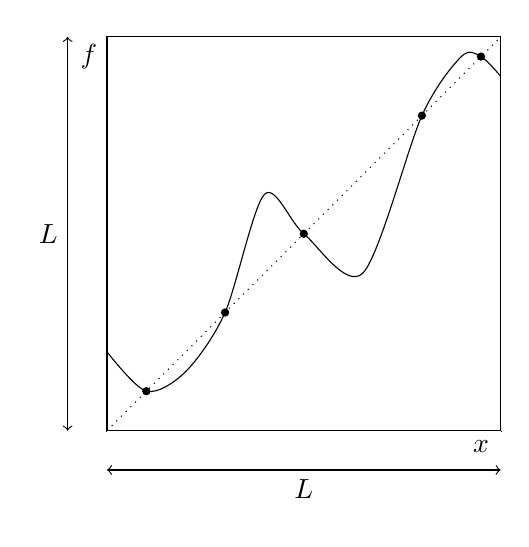
\begin{tikzpicture}[scale=1]
	
	% X
	\draw[<->] (0,-0.5)--(5,-0.5);
	\draw[<->] (-0.5,0)--(-0.5,5);
	\draw (-0.5,2.5) node[anchor=east] {$L$};
	\draw (2.5,-0.5) node[anchor=north] {$L$};

	% invisible corners
	\draw (-1,-1) node[anchor=west] {};
	\draw (5,-1) node[anchor=east] {};
	\draw (-1,5) node[anchor=west] {};

	% diagonal line
	\draw[-,dotted] (0,0)--(5,5);

	% function
	\draw plot [smooth] coordinates {(0,1) (0.5,0.5) (1,0.75) (1.5,1.5) (2,3) (2.5,2.5) (3.25,2) (4,4) (4.5,4.75) (4.75,4.75) (5,4.5)};

	% fixed points
	\fill (0.5,0.5) circle[radius=1.5pt];
	\fill (1.5,1.5) circle[radius=1.5pt];
	\fill (2.5,2.5) circle[radius=1.5pt];
	\fill (4,4) circle[radius=1.5pt];
	\fill (4.75,4.75) circle[radius=1.5pt];

	% axes
	\draw[-] (0,0)--(5,0);
	\draw[-] (0,0)--(0,5);
	\draw[-] (5,5)--(5,0);
	\draw[-] (5,5)--(0,5);

	% axis labels
	\draw (0,4.75) node[anchor=east] {$f$};
	\draw (4.75,0) node[anchor=north] {$x$};

	% fix up corners
	\fill (-0.007,-0.007) rectangle (0.001,0.001);
	\fill (5.007,-0.007) rectangle (4.999,0.001);
	\fill (-0.007,5.007) rectangle (0.001,4.999);
	\fill (5.007,5.007) rectangle (4.993,4.993);

\end{tikzpicture}